\section{Radar Cross Section}

\begin{definition}{Radar Cross Section}
    Effective area which intercepts the transmitted radar and then scatters that power isotropically back to the radar receiver.
\end{definition}

\subsection{Scattering described by Dyadics}

Scattering object eclosed by arbitrary Huygens suface $\mathcal{S}$:
\begin{itemize}
        \item Incident fields uniquely determined by tangential fields $\bs{n}\times\bs{E}_{\mathrm{inc}}$ (and $\bs{n}\times\bs{H}_{\mathrm{inc}}$) on $\mathcal{S}$
        \item Scattered fields determined by equivalent surface currents $\bs{J}_{\mathrm{sca}}$, $\bs{M}_{\mathrm{sca}}$
        \item $\bs{J}_{\mathrm{sca}}$, $\bs{M}_{\mathrm{sca}}$ = linear function of $\bs{n}\times\bs{E}_{\mathrm{inc}}$, $\bs{n}\times\bs{H}_{\mathrm{inc}}$
\end{itemize}

General linear function by integral involving scattering dyadics $\DyadicS{E}{J}$, $\DyadicS{H}{J}$, $\DyadicS{E}{M}$, $\DyadicS{H}{M}$

\begin{align}
  \bs{J}_{\mathrm{sca}}(\bs{r}) = \oiint_{\mathcal{S}} \Big[ &\DyadicS{E}{J}\GreenRs \cdot \bs{E}(\bs{r}')\nonumber\\
  &+ \DyadicS{H}{J}\GreenRs\cdot\bs{H}(\bs{r}') \Big]\,\mathrm{d}a'
\end{align}

\begin{align}
  \bs{M}_{\mathrm{sca}}(\bs{r}) = \oiint_{\mathcal{S}} \Big[ &\DyadicS{E}{M}\GreenRs \cdot \bs{E}(\bs{r}')\nonumber\\
  &+ \DyadicS{H}{M}\GreenRs\cdot\bs{H}(\bs{r}') \Big]\,\mathrm{d}a'
\end{align}

\paragraph{Redundancy} Incident fields are completely determined by tangential electric or magnetic fields alone (except resonant edge cases) $\implies$ we can discard, e.g.\, $\DyadicS{H}{J}$ and $\DyadicS{H}{M}$.

Furthermore, scattered fields can be represented by electric or magnetic currents alone, therefore e.g.\ only $\DyadicS{E}{J}$ is required.

\subsection{Polarization Scattering Matrix}
Models an incident plane wave from $\vartheta'$, $\varphi'$-direction and a scattered far-field $\bs{F}^{\mathrm{sca}}(\vartheta, \varphi) = \lim\limits_{r\to\infty} \frac{r}{e^{-jkr}} \, \bs{E}^{\mathrm{sca}}(r, \vartheta, \varphi)$.

Decomposed into co- and cross-polar components:

\begin{align}
  \begin{bmatrix}
    F_{\text{co}}^{\text{sca}}(\vartheta, \varphi)\\
    F_{\text{cr}}^{\text{sca}}(\vartheta, \varphi)
  \end{bmatrix}
  =
  \underbrace{\begin{bmatrix}
    S_{\text{co,co}}(\vartheta,\varphi,\vartheta',\varphi') & S_{\text{co,cr}}(\vartheta,\varphi,\vartheta',\varphi')\\
    S_{\text{cr,co}}(\vartheta,\varphi,\vartheta',\varphi') & S_{\text{cr,cr}}(\vartheta,\varphi,\vartheta',\varphi')\\
  \end{bmatrix}}_{\text{Polarization Scattering Matrix}}
  \begin{bmatrix}
    E_{\text{co}}^{\text{inc}}(\vartheta',\varphi')\\
    E_{\text{cr}}^{\text{inc}}(\vartheta',\varphi')
  \end{bmatrix}
\end{align}

\subsubsection{(Quasi-) Monostatic radar cross section}
\begin{itemize}
        \item Same transmit and receive antenna (or two collocated antennas) $\hat{\bs{k}} = - \hat{\bs{k}}$
        \item Fixed polarizations $\to$ only one scalar part of polarization matrix needed, e.g.\ $S_{\text{co,co}}(\hat{\bs{k}}, -\hat{\bs{k}}')$
        \item Scattered power spectrum ${|F_{\text{co}}^{\text{sca}}(\hat{\bs{k}})|}^{2} = {|S_{\text{co,co}}(\hat{\bs{k}}, \hat{\bs{k}})|}^{2} {|E_{\text{co}}^{\text{inc}}(\hat{\bs{k}})|}^{2}$
\end{itemize}
\begin{equation}
  \sigma(\hat{\bs{k}}) = 4\pi {|S_{\text{co,co}}(\hat{\bs{k}}, \hat{\bs{k}})|}^{2} \quad \text{: radar c.s.}
\end{equation}

\begin{info}{Radar Range Equation}
  \hspace{.5cm}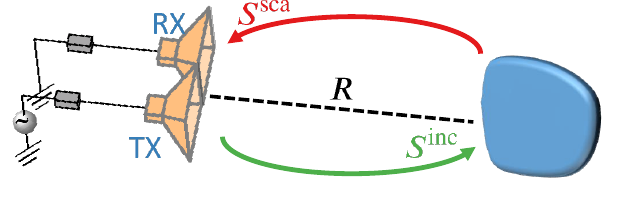
\includegraphics[width=5cm]{./content/at_meas/pictures/radar_range_eq}\\
  From the incident power at the scatterer
  \begin{equation*}
    S^{\text{inc}} = \dfrac{P_{\text{TX}}G_{\text{TX}}}{4\pi R^{2}}
  \end{equation*}
  the scattered power density of an \textit{isotropic scatterer} ($G^{\text{sca}}=1$) at antenna location
  \begin{equation*}
    S^{\text{sca}} = \dfrac{S^{\text{inc}}\sigma}{4\pi R^{2}}
  \end{equation*}
  and the received power
  \begin{equation*}
    P_{\text{RX}} = S^{\text{sca}} A_{\text{RX}}
  \end{equation*}
  the \textbf{radar range equation} is obtained
  \begin{equation}
    \dfrac{P_{\text{RX}}}{P_{\text{TX}}} = \dfrac{G_{\text{TX}}A_{\text{RX}}\sigma}{{(4\pi)}^{2} R^{4}}.
  \end{equation}
\end{info}

\subsubsection{Radar cross-section Comparison Standards}
\begin{enumerate}
        \item Perfectly conducting sphere of radius $R_{0}$
        \begin{itemize}
                \item Analytical solution for RCS via Mie Series (see lecture slides)
                \item RCS tends toward geom.\ cross section $\pi R_{0}^{2}$ for electrically large spheres
        \end{itemize}
        \item Trihedral corner reflector
        \begin{itemize}
                \item Three orthogonal surfaces $\implies$ most rays have three reflections
                \item Only three reflections for \textit{active region}
                \item Active region (normal incidence): $A = \frac{l^{2}}{2\sqrt{3}}$
                \item Radar cross section: $\sigma = \frac{\pi l^{4}}{3 \lambda^{2}}$
                \item ``Batman ears'' in response due to double-bounce echos
        \end{itemize}
        \item Less common comparision standards
        \begin{itemize}
          \item Dihedral corner plate
          \item Single plate
          \item Cylinder
        \end{itemize}
\end{enumerate}
